\section{Clasificación de objetos}  
    \subsection{Transformada de Hough}
        La transformada de Hough es usada para encontrar lineas y circunferencias en una imagen, como se ve en la figura \ref{fig:unityhough}. En el trabajo Extending Generalized Hough Transform to Detect 3D Objects in
        Laser Range Data se plantea una modificación de la transformada de Hough para usarla en espacios 3D con nubes de puntos y en lugar de buscar líneas encontrar cilindros.\\
        
        
        \begin{figure}[!htb]
            \centering
            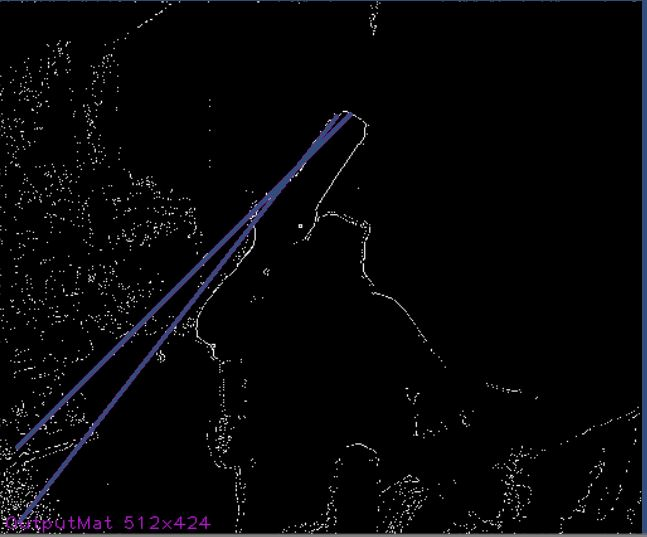
\includegraphics[width=0.6\textwidth]{02Desarrollo/RANSAC/imagenes/hough.JPG}
            \caption{Prueba de la transformada de Hough} 
            \label{fig:unityhough}
        \end{figure}
    
        Este método se descartó ya que al programar de la transformada simple de Hough en Unity3D tardo en calcular las líneas de una escena dada por el Kinect entre diez a quince segundos, y como se busca desarrollar un sistema que permita la interacción continua con el usuario el tiempo de respuesta debe ser lo más rápido posible para que la información se obtenga al momento sin tener que esperar.\\
        
    \subsection{Red Neuronal}
        El método anterior se descartó y analizó el problema desde otra perspectiva. Un método que ha dado buenos resultados en el área de visión por computadora son las redes neuronales.\\
        
        Una red neuronal es una abstracción de como se cree funciona el cerebro, teniendo como base una neurona la cual tiene estímulos de entrada y dependiendo de una función de activación envía una señal de salida. La función de activación depende de las señales de entrada y valores que se ajustan de manera automática en el entrenamiento.\\
        
        Las redes neuronales son capaces de realizar tareas de reconocimiento de manera rápida y bastante acertada, la desventaja se encuentra en el proceso de aprendizaje también llamado entrenamiento, para que la red neuronal pueda reconocer un objeto, la red debe estar entrenada para reconocer dicho objeto. Eso crea el problema de generar una base de datos de cada objeto a usar, luego realizar el entrenamiento.\\
        
        Dado a que no se cuenta con una base de datos de los objetos que se quieren representar y lo complicado que seria para el usuario agregar nuevos objetos, este método también fue descartado.
        
        
        
        
    
    
    \subsection{RANSAC}
        Como se vio en la introducción el algoritmo RANSAC se usó para estimar los parámetros de los modelos geométricos, se definieron los modelos, y los parámetros del algoritmo. Este método es preciso en la estimación de los valores de los objetos, permite estimar el tamaño, orientación y posición del objeto modelado.  \\ 
        
                
        Para atacar el problema primero se implementó RANSAC para detectar esferas como se muestra en el \gls{algoritmo} \ref{alg:RANSAC1}.\\
               
        \begin{algorithm}[!htb]
        	\caption{RANSAC}
        	\label{alg:RANSAC1}
        	\Begin{
        		k = numeroRepeticiones
        		iteraciones = 0 \\
        		n = 4
        		mejorModelo = \textbf{null}\\
        		mayorPuntosEnLaEsfera = \textbf{null}\\
        		
        		\While{iteraciones $< k$}{
        			puntosAleatorios[n] = DatosAleatoriosDe(nuevoObjeto)\\
        			nuevaEsfera = GeneraNuevaEsfera(puntosAleatorios)\\
        			puntosEnLaEsfera = []\\
        			\ForEach{ punto \textbf{in} nuevaEsfera} {
        				\If{ punto.PerteneceA(nuevaEsfera, errror $<$ t)}{
        					puntosEnLaEsfera.Add(punto)\\
        				}
        			}
        			\If{mayorPuntosEnLaEsfera.Length()$ <$ 
        			puntosEnLaEsfera.Length()}{
        				mejorModelo = nuevaEsfera\\
        				mejorPuntosEnLaEsfera = puntosEnLaEsfera\\
        			}
        			iteraciones++\\
        		}
        		\textbf{return} mejorModelo
        	}
        \end{algorithm}
    
%    
%    
%        \lstset {language=[Sharp]C}
%        \begin{lstlisting}
%iteraciones = 0;
%mejorModelo = null;
%mayorPuntosEnLaEsfera = null;
%
%while (iteraciones < k){
%    puntosAleatorios[n] =
%            DatosAleatoriosDe(nuevoObjeto);
%    nuevaEsfera = 
%            GeneraNuevaEsfera(puntosAleatorios);
%    puntosEnLaEsfera = [];
%    foreach punto in nuevoObjeto {
%        if punto PerteneceA(nuevaEsfera, errror < t)
%            puntosEnLaEsfera.Add(punto);
%    }
%    if(mayorPuntosEnLaEsfera.Length() < 
%                puntosEnLaEsfera.Length()){
%        mejorModelo = nuevaEsfera;
%        mejorPuntosEnLaEsfera = puntosEnLaEsfera;
%    }
%    iteraciones++;
%}
%return mejorModelo;
%        \end{lstlisting}
%            
%        
        Donde:
        \begin{itemize}
            \item nuevoObjeto - Nube de puntos obtenida del pre-procesamiento.
            \item n - Número mínimo de puntos para crear la esfera (4 puntos)
            \item k - Número máximo de iteraciones permitidas.
            \item t - Valor del intervalo de error permitido para determinar si un dato pertenece al modelo.
        \end{itemize}
    	
    	En el pseudocódigo las variables $mejorModelo$ y $mayorPuntosEnLaEsfera$  guardan la descripción del mejor modelo obtenido por el método RANSAC y la lista de los puntos que pertenecen a esa descripción del modelo, se inician con el valor $null$, para evitar confusiones con los otros valores, ya que $null \neq 0$, la variable $iteraciones$ encargada de contar el numero de ciclos realizados se inicia en 0, y el valor de $k$ esta dado por el numero de repeticiones que necesarias para encontrar una buena estimación del modelo, el cual se calcula mas adelante.\\
    	
        
        En este caso se uso el modelo de una \gls{esfera} en AE la cual usa cuatro puntos para describirla,  el modelo cuenta con cuatro variables a definir $(x,y,z,r)$, que corresponden al centro de la esfera y su radio, aquí es donde se obtiene el valor de la variable $n$, que esta dado por la cantidad de puntos en  $puntosAleatorios$ que son el conjunto mínimo puntos necesarios para encontrar los valores para $(x,y,z,r)$, se calcula el modelo resultante $nuevaEsfera$ usando la ecuación \eqref[ec.]{eq:esferaAE}.
        \begin{equation}
            \label{eq:esferaAE}
            \left(x-x_0\right)^2+\left(y-y_0\right)^2+\left(z-z_0\right)^2=r^2
        \end{equation}
        Para el \gls{plano} en AE se usa la forma normal de Hesse el cual consiste en la ecuación \eqref[ec.]{eq:Hesse}, donde $n$ es el vector normal al plano y $d$ es la distancia que hay del origen al plano, el signo de $d$ también determina en que dirección de $n$ se encuentra el origen, si $d>0$ entonces el origen se encuentra en la dirección de $n$, si $d<0$ el origen se encuentra en dirección contraria a $n$.
        
        \begin{equation}
            \label{eq:Hesse}
            n\cdot x=-d
        \end{equation}
        Por último para el \gls{cilindro} se usa la construcción mostrada en la ecuación \eqref[ec.]{eq:cilindro}, usando un punto base $x=(x,y,z)$ por el cual pasa un eje en dirección del vector $n=(x,y,z)$ y un radio $r$.\\
        
        \begin{equation}
        \label{eq:cilindro}
            C=\{x,n,r\}
        \end{equation}
        Los puntos $puntosAleatorios$ son elegidos de forma aleatoria y el modelo resultante $nuevaEsfera$ es comparada con cada punto en la nube de puntos para ver cuales puntos cumplen con la descripción del modelo, en otras palabras se revisa si el punto pertenece a la superficie del objeto, si es así, el punto se agrega a la lista $puntosEnLaEsfera$.\\
        
        La lista resultante se compara con la lista generada por el mejor modelo encontrado, para el primer ciclo, como aún no se tiene un modelo anterior para comparar, el modelo y la lista tienen un valor $null$, por lo cual el primer modelo calculado se guarda como el mejor modelo, que posteriormente será remplazado por alguno mejor.\\
        
        Para calcular el número de repeticiones $k$ necesarias para elegir un buen conjunto de puntos $n$, siendo $w$ la probabilidad  de que un punto seleccionado pertenece a una buena aproximación del modelo y su tolerancia de error, obtenemos la ecuación \eqref[ec.]{eq:Ek}.
        
        \begin{equation}
            \label{eq:Ek}
            E(k)= b+2*(1-b)*b+3*(1-b)^2 *b \dots+i*(1-b)^{i-1}*b+\dots
        \end{equation}
        \begin{equation}
            \label{eq:Ek2}
            E(k)= b*[1+2*a+3*a^2\dots+i*a^{i-1}+\dots] 
        \end{equation}
        Donde $E(k)$ es el valor esperado de $k$, $b=w^n$, y $a=(1-b)$.
        aplicando la identidad para series de sumas geométricas \eqref[ec.]{eq:serieSumGeo}.
        \begin{equation}
            \label{eq:serieSumGeo}
            a/(1-a)= a+a^2 + a^3 \dots+ a^i + \dots
        \end{equation}
        realizando la derivada con respecto a $a$, obtenemos la ecuación \eqref[ec.]{eq:serieSumGeoDer}.
        \begin{equation}
            \label{eq:serieSumGeoDer}
            a/(1-a)^2= 1+2*a +3*a^2 \dots+i*a^{i-1} + \dots
        \end{equation}
        obtenemos \eqref[ec.]{eq:Ek3}
        \begin{equation}
            \label{eq:Ek3}
            E(k)= 1/b=w^{-n}
        \end{equation}
        
        En la tabla \ref{tb:Ek} se muestran los valores para $E(k)$ variando los valores de $n$ y $w$, siendo $n=4$ para la esfera y $w=0.2$ serian necesarias al menos $625$ repeticiones.
    % Please add the following required packages to your document preamble:
    % \usepackage{graphicx}
    \begin{table}[!htb]
    \centering
    \caption{Valores calculados de E(k)}
    \label{tb:Ek}
    \begin{tabular}{lllllll}
    \hline
    w   & n=l & 2   & 3   & 4   & 5   & 6   \\ \hline
    0.9 & 1.1 & 1.2 & 1.4 & 1.5 & 1.7 & 1.9 \\
    0.8 & 1.3 & 1.6 & 2.0 & 2.4 & 3.0 & 3.8 \\
    0.7 & 1.4 & 2.0 & 2.9 & 4.2 & 5.9 & 8.5 \\
    0.6 & 1.7 & 2.8 & 4.6 & 7.7 & 13  & 21  \\
    0.5 & 2.0 & 4.0 & 8.0 & 16  & 32  & 64  \\
    0.4 & 2.5 & 6.3 & 16  & 39  & 98  & 244 \\
    0.3 & 3.3 & 11  & 37  & 123 & 412 & --  \\
    0.2 & 5.0 & 25  & 125 & 625 & --  & --  \\ \hline
    \end{tabular}
    \end{table}
        
        De igual manera se busca exceder el valor de $E(k)$ por una o dos derivaciones estándar. La derivación estándar $SD(k)$ esta dada por la ecuación \eqref[ec.]{eq:SDk}
        
        \begin{equation}
            \label{eq:SDk}
            SD(k)=\sqrt{E(k^2)-E(k)^2}
        \end{equation}
        Para calcular $E(k^2)$ se usa la ecuación \eqref[ec.]{eq:Ekpow2} que se obtiene de un proceso similar al usado anteriormente usando la derivación de una identidad.
        
        \begin{equation}
            \label{eq:Ekpow2}
            E(k^2)=\frac{2-b}{b^2}
        \end{equation}
        Y $SD(k)$ queda como en la ecuación \eqref[ec.]{eq:SDk2}, que para la esfera se obtiene un valor de $SD(k)=625.499\simeq 626 $, dando un valor total de repeticiones para el calculo del modelo de la esfera de $k=E(k)+SD(k)=625+626=1,250$.
        
        \begin{equation}
            \label{eq:SDk2}
            SD(k)=[\sqrt{1-w^n}]*(1/w^n)
        \end{equation}
        
        Otra forma de decidir la cantidad de repeticiones necesarias para encontrar el modelo se basa en la probabilidad. De esta forma se asegura que al menos una de las selecciones aleatorias entra en el rango de tolerancia de la predicción. Este método es el usado para el sistema ya que el número de iteraciones es menor o igual al método anterior. \\
        
        La probabilidad de encontrar el modelo deseado eligiendo $q$ puntos aleatorios se muestra en ecuación \eqref[ec.]{eq:probn}. 
        
        
        \begin{equation}
            \label{eq:probn}
            P\left(n\right)=\frac{\binom{n}{q}}{\binom{N}{q}}\approx\left(\frac{n}{N}\right)^q
        \end{equation}
        
        Donde $N$ es la cantidad de puntos en la nube de puntos, $n$ los puntos que pertenecen al modelo.\\
        
        La probabilidad de encontrar el modelo luego de $k$ iteraciones esta dada por  $P_{(n.k)}$ que se muestra  en la ecuación \eqref[ec.]{eq:probnk}. 
    
        \begin{equation}
            \label{eq:probnk}
            P\left(n,k\right)={1-\left(1-P\left(n\right)\right)}^k
        \end{equation}
        Despejando $k$ obtenemos la ecuación \eqref[ec.]{eq:probk}.
        \begin{equation}
            \label{eq:probk}
            K\geq\frac{ln(1-P_{(n,k)})}{ln(1-P(n))}
        \end{equation}
        La ecuación \eqref[ec.]{eq:probk} es calculada cada que se encuentra un mejor modelo. Entre mejor sea la representación del modelo deseado el valor $k$ será menor. El realizar el cálculo de $k$ permite terminar al algoritmo RANSAC antes de la cantidad de repeticiones estimadas con el método anterior y agilizar el algoritmo, la modificación se observa en el \gls{algoritmo} \ref{alg:RANSAC2} en las líneas [15-17]. 
        
        \begin{algorithm}
        	\caption{RANSAC modificado}
        	\label{alg:RANSAC2}
        	\Begin{
        		itreciones=0\\
        		mejorModelo=\textbf{null}\\
        		mayorPuntosEnLaEsfera = \textbf{null}\\
        		
        		\While{itreciones$ < k$}{
        			puntosAleatorios[n] = DatosAleatoriosDe(nuevoObjeto)\\
        			nuevaEsfera = GeneraNuevaEsfera(puntosAleatorios)\\
        			puntosEnLaEsfera = []\\
        			\ForEach{ punto \textbf{in} nuevoObjeto} {
        				\If{ punto.PerteneceA(nuevaEsfera, errror$ < $t)}{
        					puntosEnLaEsfera.Add(punto)\\
        				}
        			}
        			\If{mayorPuntosEnLaEsfera.Length()$ <$ 
        				puntosEnLaEsfera.Length()}{
        				mejorModelo = nuevaEsfera\\
        				mejorPuntosEnLaEsfera = puntosEnLaEsfera\\
        				
        				w = mejorPuntosEnLaEsfera/nuevoObjeto.Length()\\
        				z = 0.99\\
        				k = log( 1.0 - z )/ log( 1.0 - pow( w, n))\\
        			}
        			iteraciones++\\
        		}
        		\textbf{return} mejorModelo
        	}
        \end{algorithm}
        
        
        El valor de $z$ viene preestablecido en las bibliotecas de PCL con el valor 0.99, este valor puede ser modificado, pero al obtener un resultado aceptable se decidió no modificar los valores.
        
        
\section{Descripción General del Sistema}
        
        
    Para comprender el desarrollo de este \gls{sistema} en la figura \ref{fig:mainDiagram} se muestra el diagrama de flujo que describe el comportamiento del sistema. Se observa que son importar que datos de obtengan el sistema siempre realiza ocho procesos, los primeros cuatro procesos corresponden al pre-procesamiento en el cual se obtienen, filtran y separan los datos obtenidos del Kinect, luego se observa el cálculo de los modelos (esfera, plano y cilindro), ya sea usando AE o AGC el método se realiza de la misma manera para luego compararlos dependiendo de cual describe mejor a al conjunto de datos obtenidos, para el uso de AGC los puntos fueron transformados del espacio euclidiano $\mathbb{R}^{3}$ al espacio $\mathbb{R}^{n+1,1}$, así como las figuras obtenidas usando AGC fueron interpretadas para su representación en el espacio euclidiano.
    \clearpage
    \begin{figure}[!htb]
       	\centering
       	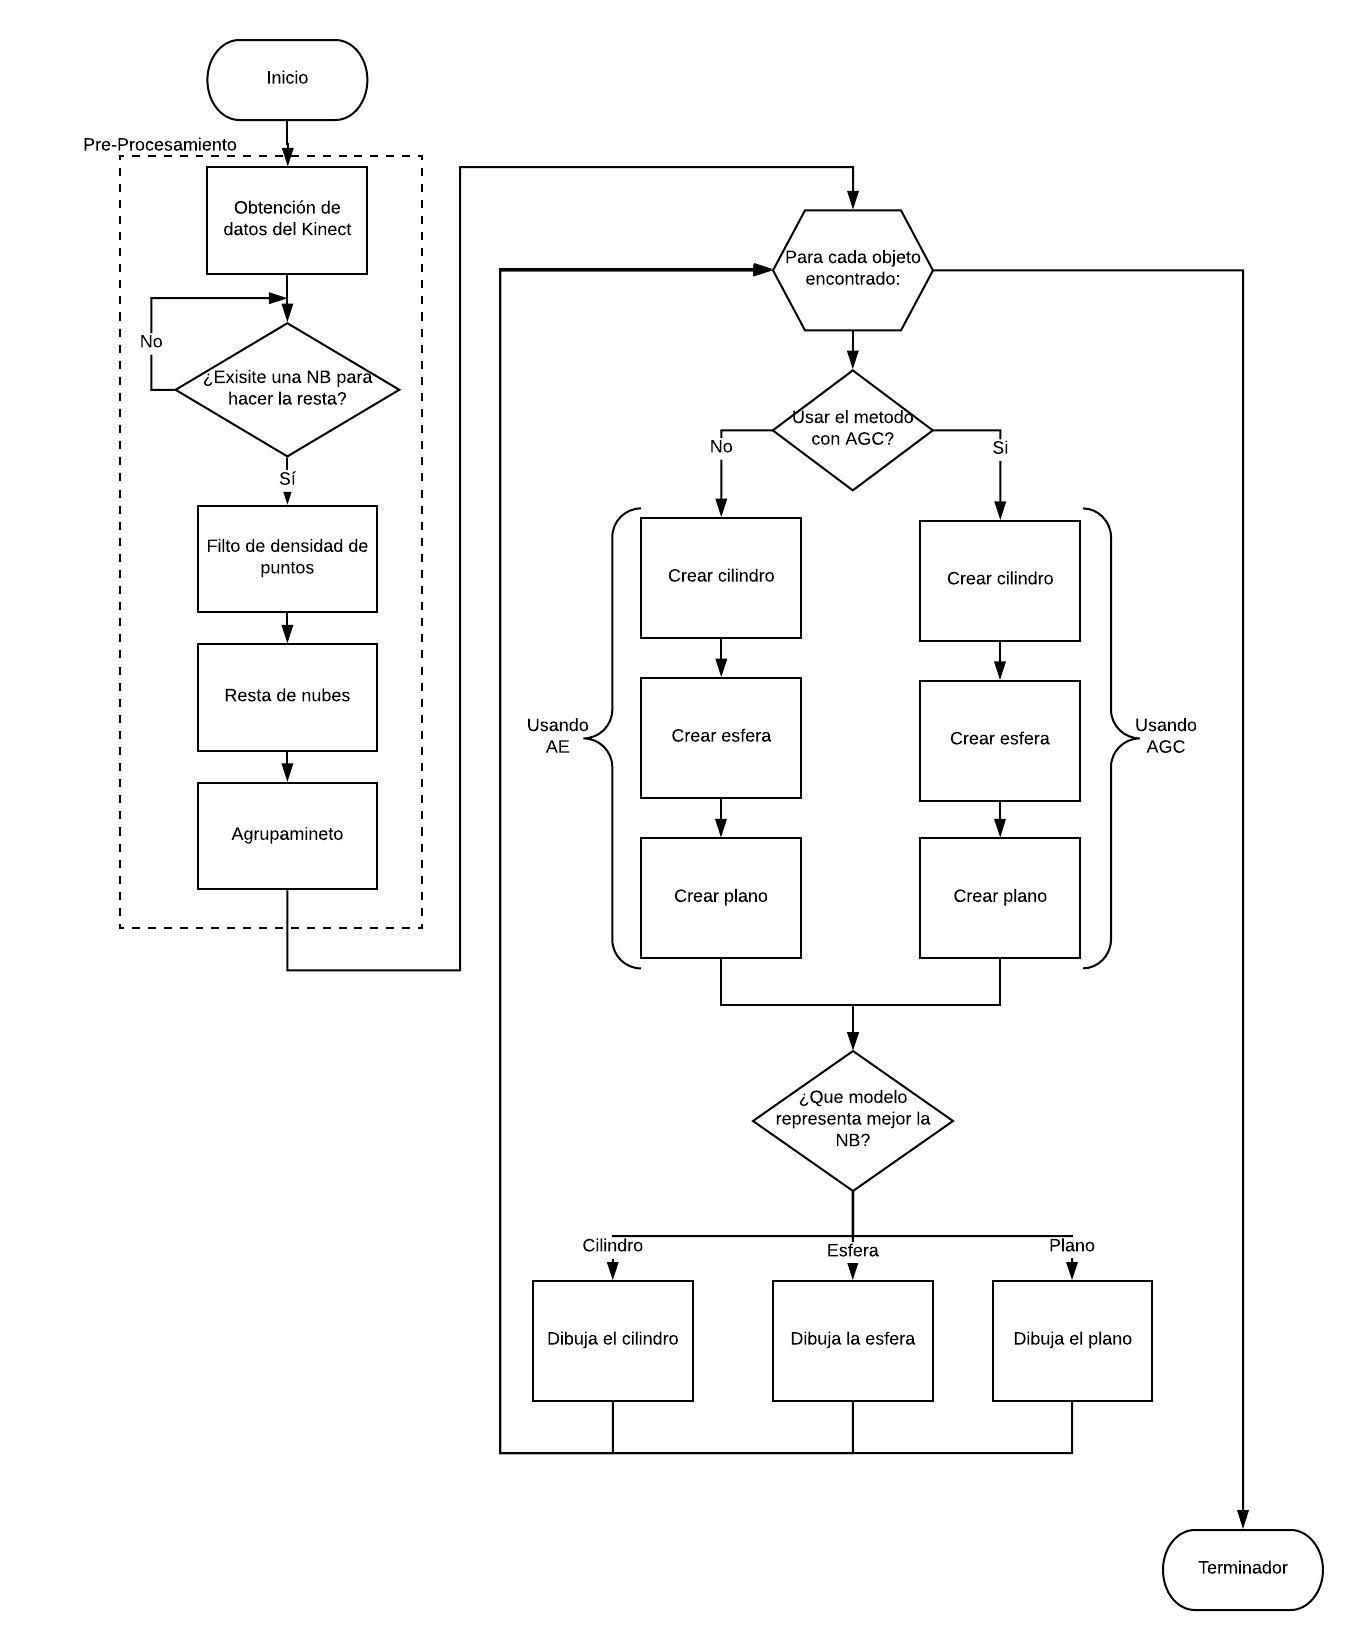
\includegraphics[width=\textwidth]{02Desarrollo/RANSAC/imagenes/MainGiagram2.jpeg}
       	\caption{Diagrama de flujo del sistema} 
       	\label{fig:mainDiagram}
    \end{figure}